\documentclass[11pt]{article}
\title{Technical Report\\ COMP1100 Assignment 2}
\author{Jacob Bos\\ ANU u7469354}

\usepackage{graphicx}
\usepackage{amsmath}
\usepackage{amssymb}
\usepackage{array}
	\newcolumntype{L}{>{\centering\arraybackslash}m{15cm}}
\usepackage{float}
\usepackage{multicol}
\setlength{\columnsep}{1cm}
\usepackage{setspace}
\usepackage{xcolor}

\newenvironment{smallpmatrix}
  {\left(\begin{smallmatrix}}
  {\end{smallmatrix}\right)}
 \newenvironment{smol}
  {\left(\begin{smallmatrix}}
  {\end{smallmatrix}\right)}


\usepackage[margin=2cm]{geometry}
\addtolength{\textheight}{-0.5cm}
%~~~~~~~~~~~~~~~~~~~~~~~~~~~~~~~~~~~~~~~~~~~~~~~~~~~~~~~~~~~~~~~~~~~~~~~~~~~~~~~~~~~~~~~~~~~~~~~~~~~~
%~~~~~~~~~~~~~~~~~~~~~~~~~~~~~~~~~~~~~~~~~~~~~~~~~~~~~~~~~~~~~~~~~~~~~~~~~~~~~~~~~~~~~~~~~~~~~~~~~~~~
\begin{document}
\maketitle
\pagenumbering{roman}
\setstretch{1.5}
\begin{center}
  Lab: Tuesday 11am\\
  Tutor: Abhaas Goyal\\
  Word-count beyond cover page at $\leq 1250$ words
\end{center}
\tableofcontents
\newpage
\pagenumbering{arabic}
%~~~~~~~~~~~~~~~~~~~~~~~~~~~~~~~~~~~~~~~~~~~~~~~~~~~~~~~~~~~~~~~~~~~~~~~~~~~~~~~~~~~~~~~~~~~~~~~~~~~~
\section{Introduction} 
The program detailed herein is an implementation of Fransson's \textit{QR World} cellular automata and graphical representation in Haskell with complimentary unit tests.


%~~~~~~~~~~~~~~~~~~~~~~~~~~~~~~~~~~~~~~~~~~~~~~~~~~~~~~~~~~~~~~~~~~~~~~~~~~~~~~~~~~~~~~~~~~~~~~~~~~~~
\section{Documentation}%Explanation of code workings, functions and structure.
\subsection{Design Documentation and Technical Decisions}
% Describe what each relevant function does conceptually. (i.e. how does it get you closer to solving the problems outlined in this assignment spec?)
% How do these functions piece together to make the finished program? Why did you design and implement it this way?
% What major design choices did you make regarding the functions that you’ve written and the overall structure of your program?
\paragraph{Task 1}  defined the type of  \verb|QRCell| as either \verb|Dead| or \verb|Alive|.  An if then else (ITE) statement is used for \verb|toQR| to convert values in a textual representation to useful values with \verb|'A'| becoming \verb|Alive::QRCell| and anything else returning \verb|Dead|. \verb|cycleQR| swaps a cell's state upon cursor clicks using a case statement. \verb|renderQR| renders each cell as a codeWorld picture. \verb|get| retrieves the cell's value for a given \verb|GridCoord|, returning \verb|Nothing| for nonsensical arguments. \verb|allCoords| generates a row-major list of all coordinates in an $(a\times b)(a,b>0)$ grid returning an error for nonsensical arguments of $a,b\not>0$ as par specifications. Otherwise it calls 3 helper functions. \verb|nList| generates an ascending list from 0 to (a-1). \verb|nPair| then pairs each value in  \verb|nList| with some integer. \verb|allPairs| then uses \verb|nList|to create one list from (0,0) to (a-1,b-1). 

\paragraph{Task 2} consists of two primary functions, \verb|nextGenQR| which parses the automata through one iteration, and \verb|evolveQR| which iterates the automata $n$ times. \verb|nextGenQR| calls  \verb|allCoords| and \verb|nextGenQrGrid|, which is the main function handling the grid evolution. \verb|nextGenQrGrid| recurses through the \verb|allCoords| list with \verb|get| retrieving the state at each position and \verb|findHood| retrieving a list of the neighbouring states. \verb|decideEvolve| updates the state of the cell according to the QRWorld rules. This new state is then prepended to the recursive call on the rest of the \verb|allCoords| list. \verb|allCoords| is guarded to return an error for nonsensical grid dimensions avoiding irrational program operation. A guarded case recursion was chosen for \verb|countAlive| to only count alive elements. \verb|decideEvolve| was chosen to use a case to direct the function to guards based on the number of alive neighbours determined by \verb|countAlive| to then decide how to change  the state. \verb|findHood| uses \verb|get| to retrieve a four element list of \verb|[Maybe QRCell]| to give the states of the neighbouring cells. \verb|decideEvolve| then calls \verb|countAlive| to then make a decision about what each cell state should evolve to depending on how many alive neighbours it has. To do this it cases on the state of the cell and is then guarded by the number of alives to evolve the state properly. \verb|countAlive| just uses a case and nested guard recursion to sort through the list of neighbouring states and returns the number that are alive. \verb|evolveQR| recurses down to a base of 1 from a natural $n$ applying \verb|nextGenQR| to itself $n$ times.

\newpage
\subsection{Program Design / Structure}
The following is a module and function dependency graph for the program and test program: 
  \begin{figure}[H]
    \centering
    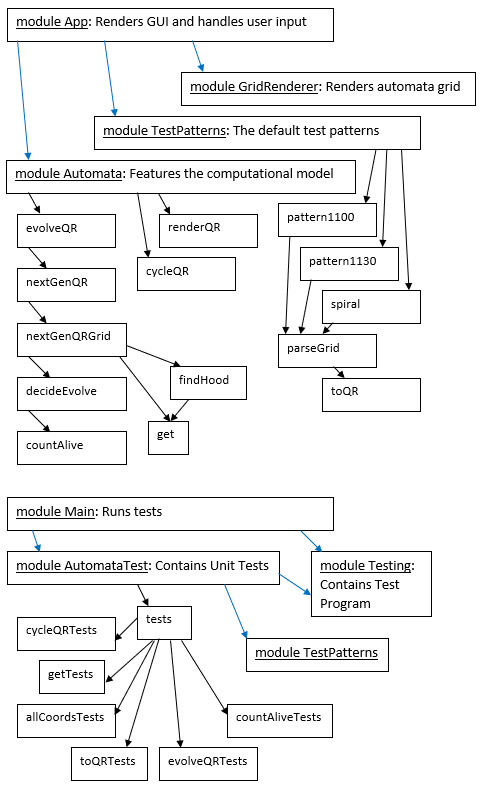
\includegraphics[width=0.65\textwidth]{funcDep.png}
  \end{figure}
  \newpage
  The program's broad structure was dictated by the specifications with modules and key functions already named and structured. The above graph mostly shows the functions developed by the author and their helper functions.  The author broke \verb|allCoords| up into helper functions for ease of understanding, allowing a clear step by-step construction of the list with \verb|allCoords| just calling the helper functions that do each construction.\\
  
   It was chosen that \verb|nextGenQR| would have a helper \verb|nextGenQRGRid| because the former was unable to recurse through a list of \verb|allCoords| but the latter could be made to. This ability was important as it made it easier to maintain the order of the state list  and aided the implementation of \verb|findHood| which was needed to make the evolution decision for each cell. Designing \verb|findHood| to return a list rather than a 4 element double was chosen as it allowed \verb|countAlive| to use recursion which Haskell is optimised for.\\
   
   It was chosen that the main test function would concatenate separate test functions of type \verb|[Test]| together to allow easier documentation via comments and function naming. 

 \subsection{Assumptions}%Describe assumptions you have made about how a user might use the program and how this has influenced your design decisions.
Whilst writing \verb|get| it was assumed that attempts to retrieve a point outside the grid should return \verb|Nothing :: Maybe QRCell| as doing so eased implementation of \verb|findHood| and \verb|countAlive| far more than returning an error would. It was initially assumed that nonsensical inputs to \verb|allCoords| should return an empty list but this was revised to return an error as specified.

%~~~~~~~~~~~~~~~~~~~~~~~~~~~~~~~~~~~~~~~~~~~~~~~~~~~~~~~~~~~~~~~~~~~~~~~~~~~~~~~~~~~~~~~~~~~~~~~~~~~~

\section{Testing}%How did I test the program focus on methodology and testing groups
%How did you test individual functions?
%Be specific about this - the tutors know that you have tested your program, but they want to know how.
%Describe the tests that prove individual functions on their own behave as expected (i.e. testing a function with different inputs and doing a calculation by hand to check that the outputs are correct).
%How did you test the entire program? What tests did you perform to show that the program behaves as expected in all (even unusual) cases?
\paragraph{Unit tests} were divided into 6 groups, each testing a particular function and/or their helpers. \verb|cycleQRTests| is a fully comprehensive test group for \verb|cycleQR| indicating its correctness. \verb|toQR| is tested against tests two typical cases and an edge case. The tests for \verb|get| cover most possible edge cases and also some typical cases as documented in the \verb|AutomataTest| file. The tests for \verb|allCoords| covers some expected inputs to both the main function and helpers. There were no edge case tests written as such cases are written to return an error and there was no provision to test if errors are returned.\\

 \verb|evolveQR| was tested with three unit tests which also test \verb|nextGenQR| due to \verb|evolveQR|'s dependency. The first two check if the 1100 pattern gets to an alternating steady state after 12 evolutions and the third if the 1130 pattern eventually reached steady state as specified. All tests passed indicating program correctness. All these tests are documented with comments in \verb|AutomataTest.hs|
 
\paragraph{GUI tests} focussed on the behaviour of functions which handle direct user interaction. \verb|get| and \verb|cycleQR| were tested by clicking cells with various states and checking if the appropriate cell switched state. \verb|decideEvolve| was tested by observing the evolution of a single cell in various neighbourhoods compared against the rules of QRWorld. All tests passed indicating correctness.
%~~~~~~~~~~~~~~~~~~~~~~~~~~~~~~~~~~~~~~~~~~~~~~~~~~~~~~~~~~~~~~~~~~~~~~~~~~~~~~~~~~~~~~~~~~~~~~~~~~




\section{Reflection}
%Discuss the reasoning behind your decisions, rather than what the decisions were. You can reflect on not only the decisions you made, but the process through which you developed the final program:
   %What would you have done differently if you were to do it again
    %What changes to the design and structure you would make if you wrote the program again from scratch?
    \subsection{Design Choices}
   Program development followed progressed linearly parallel to ordering of the specifications.  Design decisions were made with both functionality and style in focus, making proper use of Haskell's recursive propensity. Consequently, program is quite readable and supplemented by effective documentation comments.\\
   
   ITE statements were used whenever it was necessary to check for one case and return a single answer for anything else. Guard and case recursion was selected based on whether the function needed to iterate n times or traverse a list. For \verb|allPairs| and \verb|nList| which iterate n times, (++) allowed proper order of the list as n counts down but the list counts up. When traversing a list (:) was used to maintain the input ordering such as for  \verb|nPair|. \\
   
   An algebraic datatype was chosen for \verb|QRCell| as it was more descriptive of the program's meaning than boolean values. \verb|renderQR| uses a piecewise definition to improve style. Guards were chosen for \verb|get| to protect against retrieving elements outside the automata grid.  It was chosen for \verb|nextGenQR| to call \verb|nextGenQrGrid| so that the helper functions could be called appropriately and allow for a recursion through the list of \verb|allCoords|.

   \subsection{Reflection}
   If they were to re-develop the program the author believes the helper  \verb|nPair| could be rewritten or removed by using \verb|map| and \verb|(\y x -> (x,y))|. However, they would make no changes to the structure which was largely dictated largely by specifications.\\
   
   The program was within the author's technical abilities and so no significant problems encountered in development however, they suspect that there is a cleaner way to write \verb|allCoords| as it is rather convoluted, however, other than what's mentioned above, inspiration escapes them. The author had some trouble defining the type \verb|QRCell| but came to a good solution under closer reading of the specifications which allowed the rest of the program to develop smoothly. Consequently, they did not need to collaborate with others in any significant way.




%~~~~~~~~~~~~~~~~~~~~~~~~~~~~~~~~~~~~~~~~~~~~~~~~~~~~~~~~~~~~~~~~~~~~~ ~~~~~~~~~~~~~~~~~~~~~~~~~~~~~~~


%~~~~~~~~~~~~~~~~~~~~~~~~~~~~~~~~~~~~~~~~~~~~~~~~~~~~~~~~~~~~~~~~~~~~~~~~~~~~~~~~~~~~~~~~~~~~~~~~~~~~
\end{document}